\documentclass[11pt,a4paper,oneside,table,xcdraw]{article}

% CREATED BY DAVID FRISK, 2015


% BASIC SETTINGS

\usepackage{url}
\usepackage{lastpage}								% Get the number of pages
\usepackage{moreverb}								% List settings
\usepackage{textcomp}								% Fonts, symbols etc.
\usepackage{lmodern}								% Latin modern font
\usepackage{helvet}									% Enables font switching
\usepackage[T1]{fontenc}							% Output settings
\usepackage[english]{babel}							% Language settings
\usepackage[utf8]{inputenc}							% Input settings
\usepackage[table]{xcolor} 							% Table colors
\definecolor{light-gray}{gray}{0.96}			% Defining a very light gray for a table

\usepackage{amsmath}								% Mathematical expressions (American mathematical society)
\usepackage{amssymb}								% Mathematical symbols (American mathematical society)
\usepackage{graphicx}								% Figures
\usepackage{subfig}									% Enables subfigures

\usepackage{listings}								% Enables source code listings
\usepackage{xparse}								% Enables in-line code
\NewDocumentCommand{\codeword}{v}{ % Enables in-line code
	\texttt{\textcolor{blue}{#1}}
}
\usepackage{chemfig}								% Chemical structures
\usepackage[top=3cm, bottom=3cm,
			inner=3cm, outer=3cm]{geometry}			% Page margin lengths			
\usepackage{eso-pic}								% Create cover page background
\newcommand{\backgroundpic}[3]{
	\put(#1,#2){
	\parbox[b][\paperheight]{\paperwidth}{
	\centering
	\includegraphics[width=\paperwidth,height=\paperheight,keepaspectratio]{#3}}}}
\usepackage{float} 									% Enables object position enforcement using [H]
\usepackage{parskip}								% Enables vertical spaces correctly 
\usepackage{minted}
%Code highlighting and formatting
\usepackage{dirtree}
\usepackage{epigraph}
%Appendix
\usepackage[toc,page]{appendix}
\usepackage{wrapfig}
\usepackage{caption}
% OPTIONAL SETTINGS (DELETE OR COMMENT TO SUPRESS)

% Disable automatic indentation (equal to using \noindent)
\setlength{\parindent}{0cm}                         


% Caption settings (aligned left with bold name)
% \usepackage[labelfont=bf, textfont=normal,
%			justification=justified,
%			singlelinecheck=false]{caption} 		

		  	
% Activate clickable links in table of contents  	
\usepackage{hyperref}								
\hypersetup{colorlinks, citecolor=black,
   		 	filecolor=black, linkcolor=black,
    		urlcolor=black}


% Define the number of section levels to be included in the t.o.c. and numbered	(3 is default)	
\setcounter{tocdepth}{5}							
\setcounter{secnumdepth}{5}	


% Chapter title settings
\usepackage{titlesec}		
\titleformat{\chapter}
  {\Large\bfseries}{{\fontsize{35pt}{1em} {\thechapter}}}{1ex}{}[]


% Header and footer settings (Select TWOSIDE or ONESIDE layout below)
\usepackage{fancyhdr}
\pagestyle{fancy}
\fancypagestyle{plain}{}
\lhead{}
\rhead{}
\renewcommand{\chaptermark}[1]{\markboth{\thechapter.\space#1}{}}


\fancyhf{}
\fancyhead[L]{Rasmus Isager Kruuse\\Human senses and perception miniproject}
\fancyhead[R]{15/01 - 2018\\MED3}
\fancyhead[C]{}
\fancyfoot[C]{\thepage}

\usepackage[final]{pdfpages}
\usepackage{verbatim}
\usepackage{lipsum}
\usepackage{multicol}
% Enable To-do notes
\usepackage[textsize=tiny]{todonotes}   % Include the option "disable" to hide all notes
\setlength{\marginparwidth}{2.5cm} 

\usepackage{tikz}
\usetikzlibrary{mindmap,trees}
\usepackage{nameref}

% Supress warning from Texmaker about headheight
\setlength{\headheight}{30pt}		

\newcommand{\HRule}{\rule{\linewidth}{0.5mm}}

\usepackage[normalem]{ulem}
\useunder{\uline}{\ul}{}

\usepackage{tocbibind}

\usepackage{tikz}
\usepackage{pgf-pie}
\usepackage{pgfplots}
\pgfplotsset{width=12cm,compat=1.11}
\pgfplotsset{
	cycle list={red\\blue\\},
}
\usepgfplotslibrary{statistics}




\usepackage[natbibapa]{apacite} 
\usepackage[export]{adjustbox}

\begin{document}

\begin{titlepage}
\newgeometry{top=3cm, bottom=3cm,
			left=2.25 cm, right=2.25cm}	% Temporarily change margins		
			
% Cover page background 
\AddToShipoutPicture*{\backgroundpic{-4}{56.7}{figure/Frontpage/frontpage-aau.pdf}}
\addtolength{\voffset}{2cm}

% Cover picture 		
\begin{figure}[H]
\centering
\vspace{2cm}	% Adjust vertical spacing here
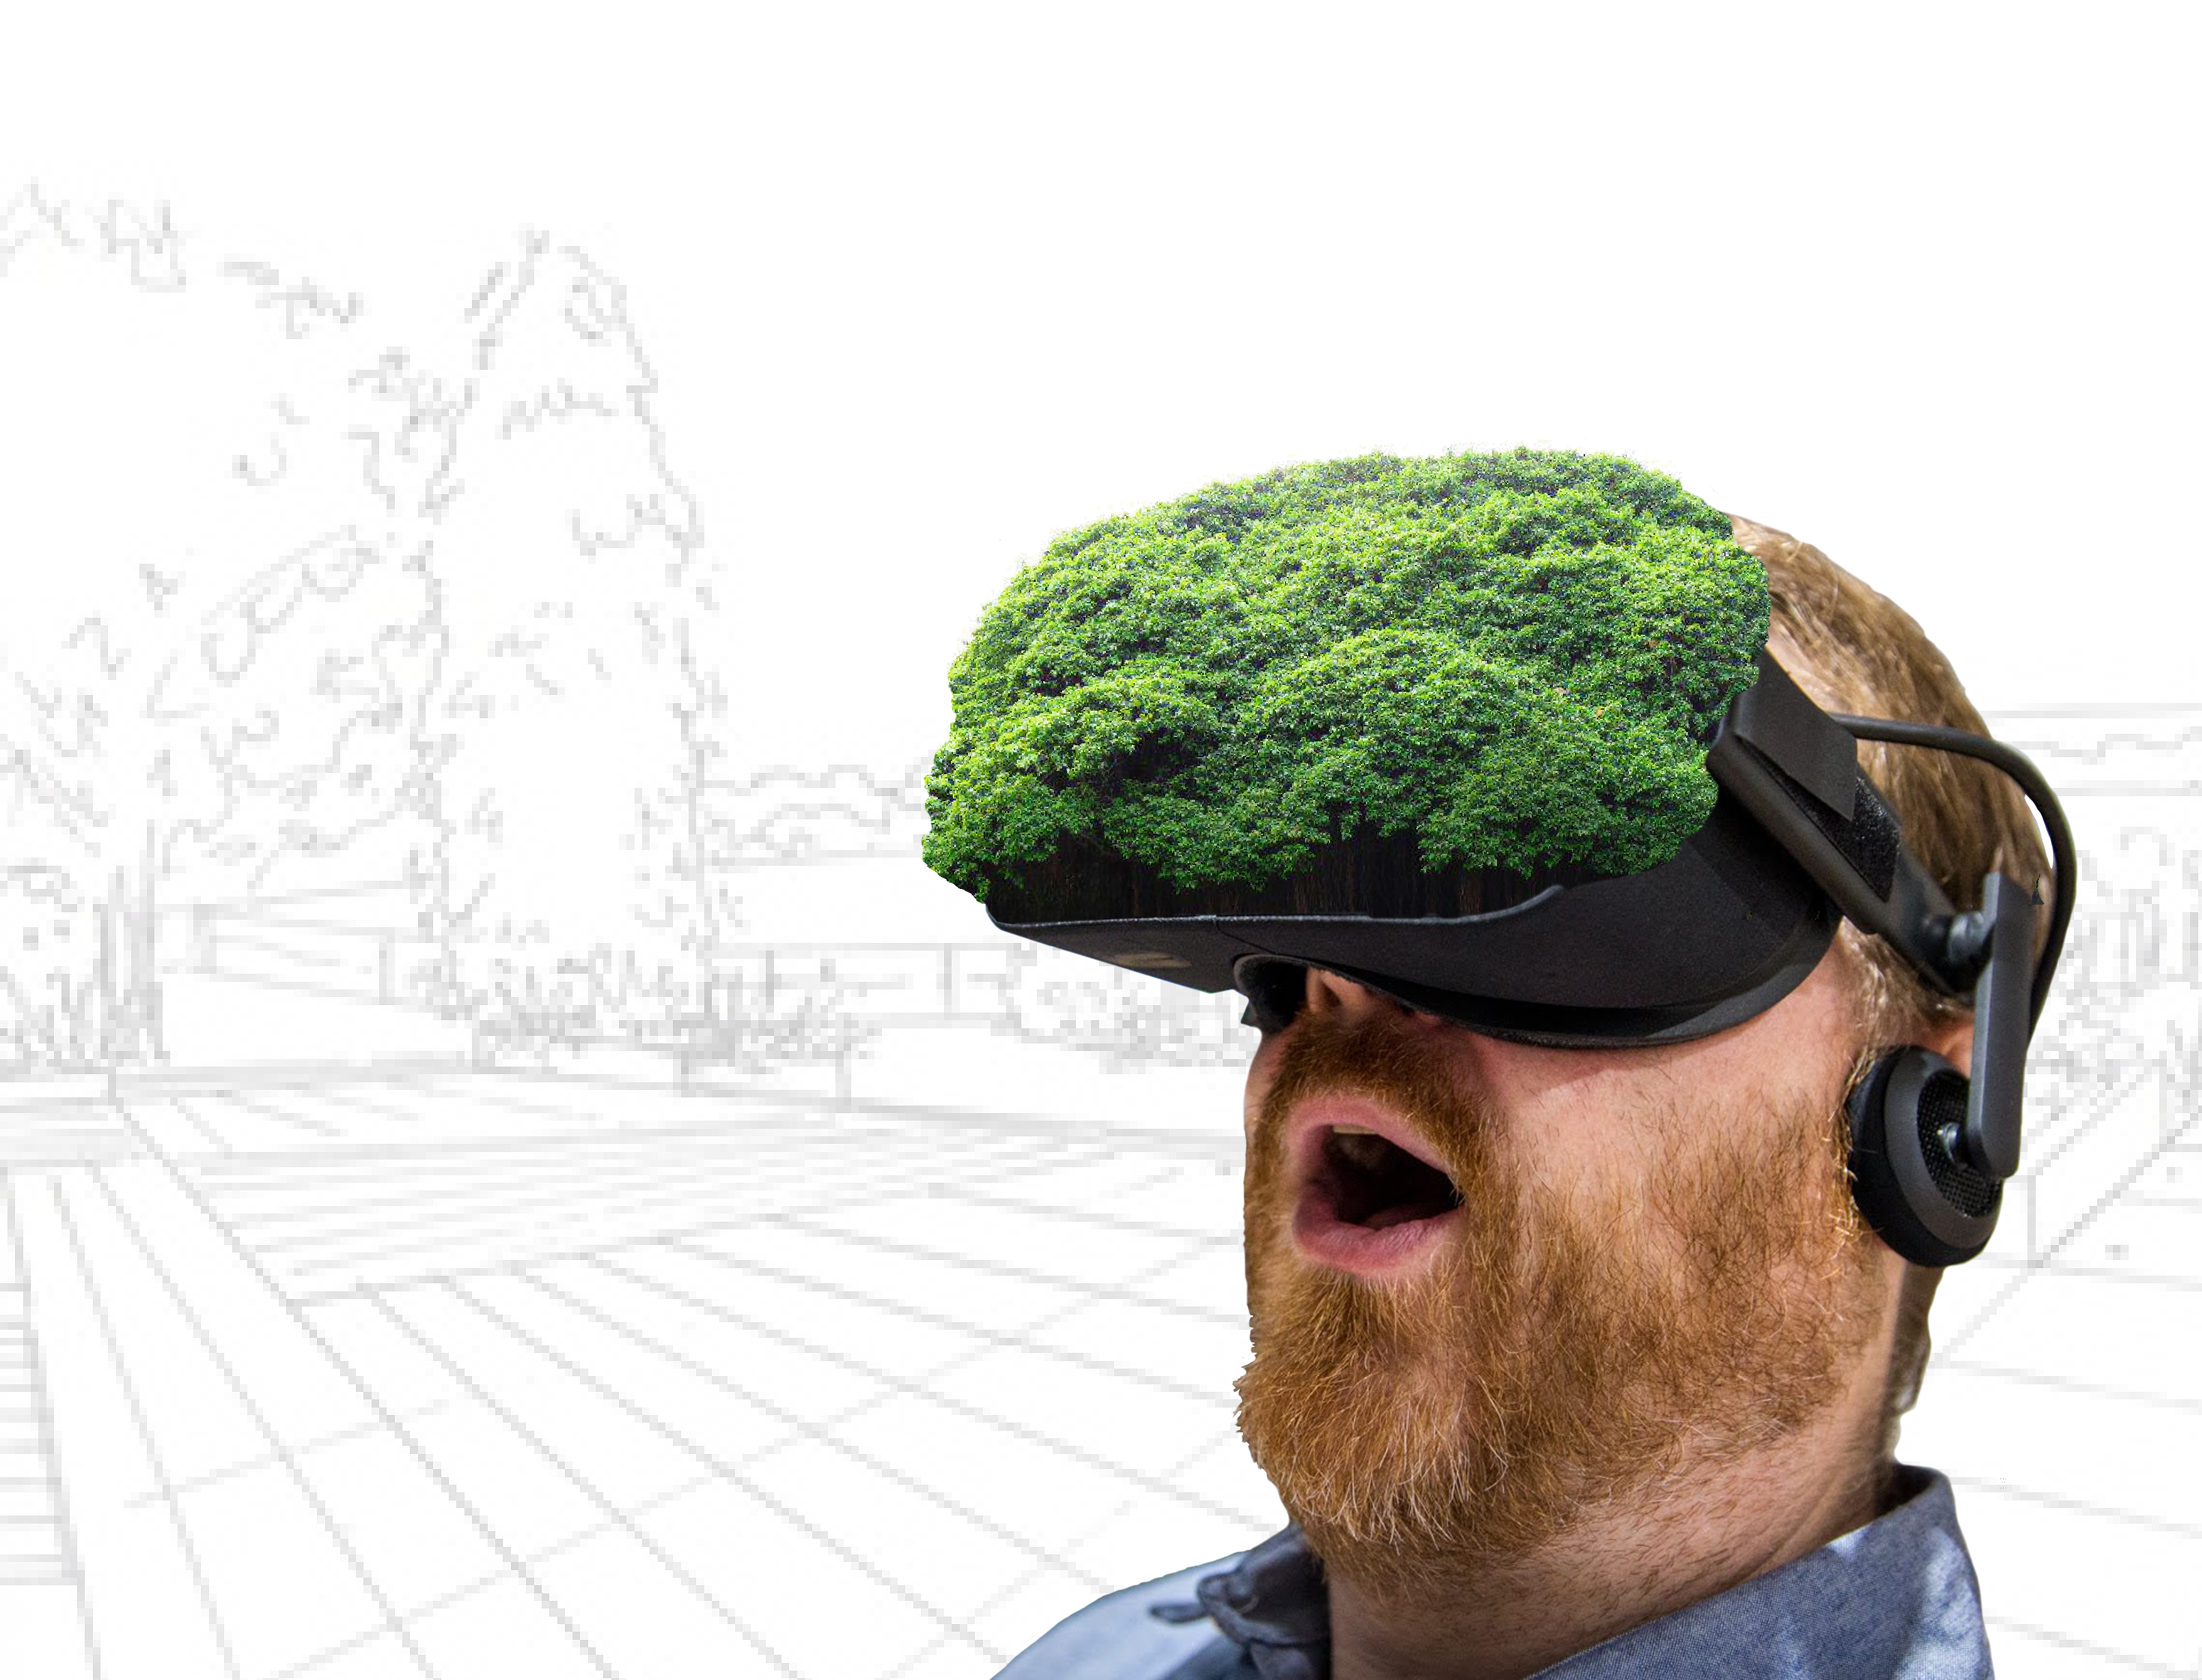
\includegraphics[width=0.99\linewidth]{figure/Frontpage/gardenposterCropped.png}
\end{figure}

% Cover text
\mbox{}
\vfill
\renewcommand{\familydefault}{\sfdefault} \normalfont % Set cover page font
\HRule\\[0.1cm]
\textbf{{\small Human Senses and Perception\\ {\Huge Vection}}} \hspace{0.15cm}\hspace{0,15cm}{\huge \color{gray}and other types of illusory motion}\\
\HRule\smallskip{}

\Large by \LARGE Rasmus Isager Kruuse\\
\Large stdnr: 20163929\\\\


\today
\renewcommand{\familydefault}{\rmdefault} \normalfont % Reset standard font
\end{titlepage}




\pagenumbering{arabic}

\section{Introduction - what is vection}
You are sitting on a train waiting at the station, zoned out, staring into the middle distance. When your trains set in motion, it takes you a few seconds to realize that it was actually the train across from you that moved. Your brain played tricks on you. This trick is called vection, and everyone has experienced it at some point in thier life. This paper aims to explain why vection happens, by introducing the relevant theory and and goes on to compare vection to other types of illusory self motion. Finally it discusses the relevancy of vection as it relates to media technology. 
\section{What \textit{is} vection?}
\label{sec:def}
One of the problems with the term vection, is that it has been used to describe many different things by different researchers. \cite{challenges} published a paper in which they stated four challenges that vection research currently faces. One of these is the lack of a concrete definition. They gave examples of four different definitions that was used in research. To prevent this, vection is defined early in this paper and is based on the description of vection provided by \cite{vection}.
\begin{quote}
\textit{When we are exposed to a visual motion field that simulates the retinal optical flow generated by our movement, we often perceive subjective movement of our own bodies. This phenomenon is called vection.}
\end{quote}
I base my definition on this, because other definitions, such as the ones provided by \cite{challenges} are either too narrow (being limited to stationary vision) or too broad (describing both real and illusory motion). As such the definition used in this report is.
\begin{quote}
\textit{\textbf{Vection} is a simulation of the optical flow generated by movement, that causes perceived self motion}
\end{quote}
To understand how optic flow can trick the human perception system into feeling self motion where there is none, we must first understand what optic flow is, how it is used in motion perception, and why this causes no problems under normal conditions.
\section{Theory of optic flow}
This section covers the theory of optic flow relevant for vection.
%\todo{Answer the following questions 3. Vection. Explain what vection is and how it differs from other types of illusory self motions one might experience. When and how can we experience vection? What determines whether it happens or not and how long the sensation lasts? }	
\subsection{Optic flow}
Every point in a persons field of view can be mapped to a position on the retina in one of the eyeballs. If the person moves or looks in a different direction, or if the thing causing that point moves, the points position on the retina changes. This is illustrated in Figure \ref{fig:eye}\todo{adjust figure}.
\begin{figure}[H]
		\centering
		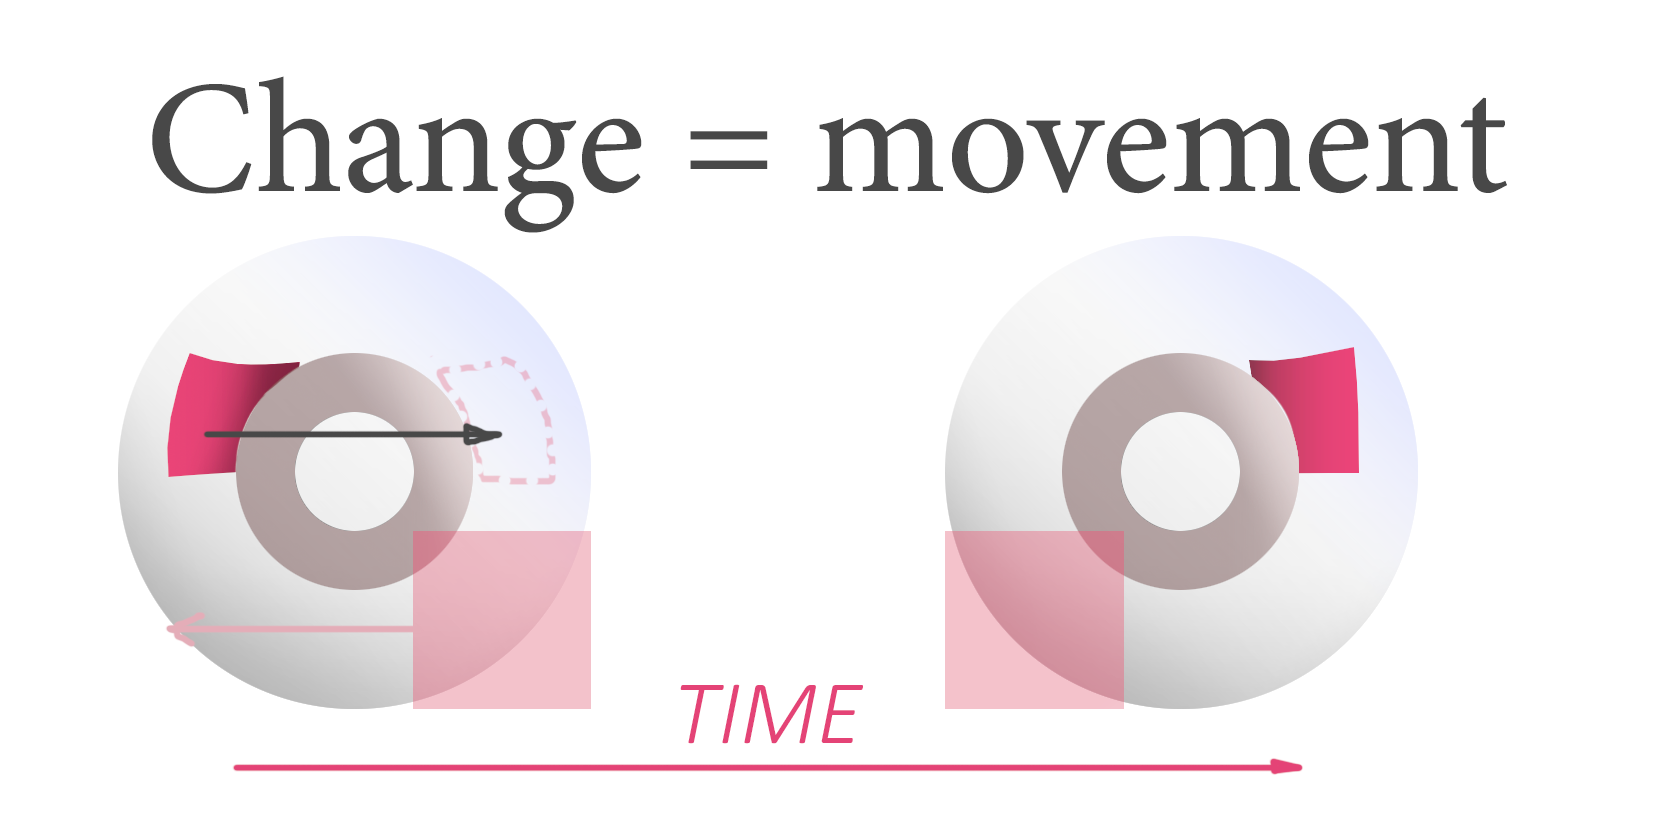
\includegraphics[width=0.7\linewidth]{figure/eyes.png}
		\caption{Movement of the purple square outside of the eye cause the image that it casts on the back of the eye to move correspondingly}
		\label{fig:eye}
\end{figure}
In all cases, global changes happens to the light that the eyes receive. In the example shown in Figure \ref{fig:opticalflow}, during forward movement, objects and by extension the light they cast, tends to move away from the center of the eye. These structural changes are called called optic flow, and can be used to estimate heading (\cite{opticflowheading}), and are a powerful cue in motion perception (\cite{opticalflow}).
\begin{figure}[H]
		\centering
		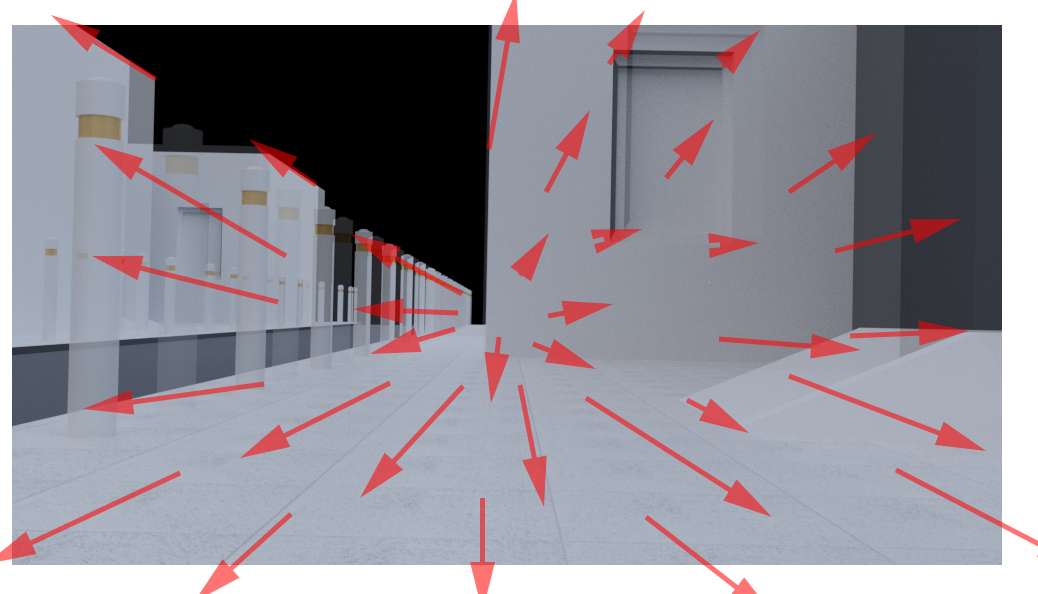
\includegraphics[width=0.8\linewidth]{figure/opticalflow.png}
		\caption{During forward movement, the optic flow is expanding. Human vision use these large scale similar changes to estimate direction.}
		\label{fig:opticalflow}
\end{figure}
Optic flow is not limited to forward or backwards movement. A person turning their head will see optic flow in the opposite direction to rotation. However, what if only the eyes move? There would be no motion, but the points would still move on the retina. Will this not cause the brain to experience flow even though neither you or the object is moving? The brain avoids this issue by sending a copy of the motor commands, known as the CD (corollary discharge) to the visual system (\cite{schcd}). The CD can be used to correct for changes that happen during eye movement \cite[p. 241-242]{coursebook}. As such, optic flow on the retina provide reliable cues for both rotation and movement, while ignoring "fake" movement that happens when they eyes move.\\
Models have been suggested that are able to track luminance changes on the retina over time (\cite{opticflowheading}). While the output of a single cell behaving after this model is unreliable, the combined output of many could form the basis for how optic flow is detected early in the vision system (\cite{schopticflow}).
\subsection{Vision based motion detection}
Since a three dimensional world is projected onto a two dimensional surface (the retina), motion can be though of as an image moving around the retina. If a point is somewhere at one time, and elsewhere at another, it must have moved. In the retina there are light sensitive cells that respond to light. The output from a number of these can be combined to detect local changes in light, and respond strongly to edges \cite[p. 53]{coursebook}. The section of vision that these cells are responsible for is called their \textit{receptive fields}. Thinking of motion in terms of receptive fields, if one receptive field gives a powerful response, and a few milliseconds later a nearby receptive field also gives a powerful response. Then perhaps whatever caused that response has moved, as illustrated in Figure \ref{fig:overtime}.
\begin{figure}[H]
		\centering
		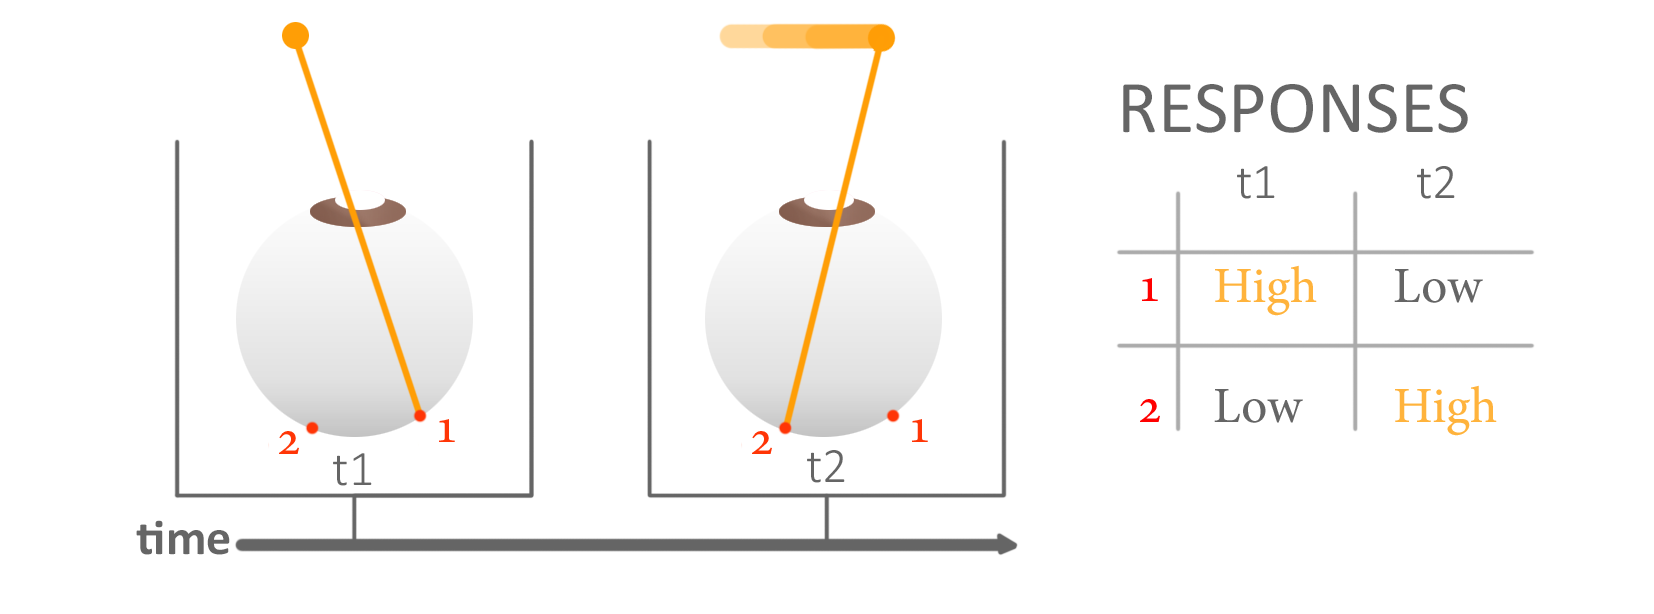
\includegraphics[width=1\linewidth]{figure/overtime.png}
		\caption{In terms of the eye, movement can be though of as different receptive fields showing high responses at different times. Here at time 1 light from an object hits point 1. Later at time 2 the object has moved and the light from it now its point 2. As such if one wanted to track the object, one would track how the light from it travels across the back of the eye over time}
		\label{fig:overtime}
\end{figure}
The retina has around 1 million receptive fields covering the eye's field of view, with many of the field types overlapping  \cite[p. 64-65]{coursebook}. \cite{Barlow1965} found cells in the retina of rabbits, that gave a powerful responses when an object moved through a specific part of the rabbit's vision in one direction, but would give little to no response if the object was moved in the opposite direction. These were named direction sensitive cells, or DS cells. \citet{review} points out that multiple models have been suggested that could explains this behaviour. They rely on combining the output of multiple receptive fields.\\\\
The receptive field can in the context of this report be though of light bulbs, that are ON (fire) when light hits them, and otherwise are off. If we imagine a neuron N that is connected to two receptive fields f1, and f2. This neuron, N, will only fire if it simultaneously receives a signal from both receptive fields. If an object moves across each of the receptive fields in succession. The first field (f1) will fire, and then the second (f2) will fire. However, by the time the signal from f2 reaches N, the signal from f1 has already arrived. This problem is illustrated in Figure \ref{fig:nodelay}. Because the signals do not arrive at the same time, N will not fire.
\begin{figure}[H]
\begin{multicols}{2}
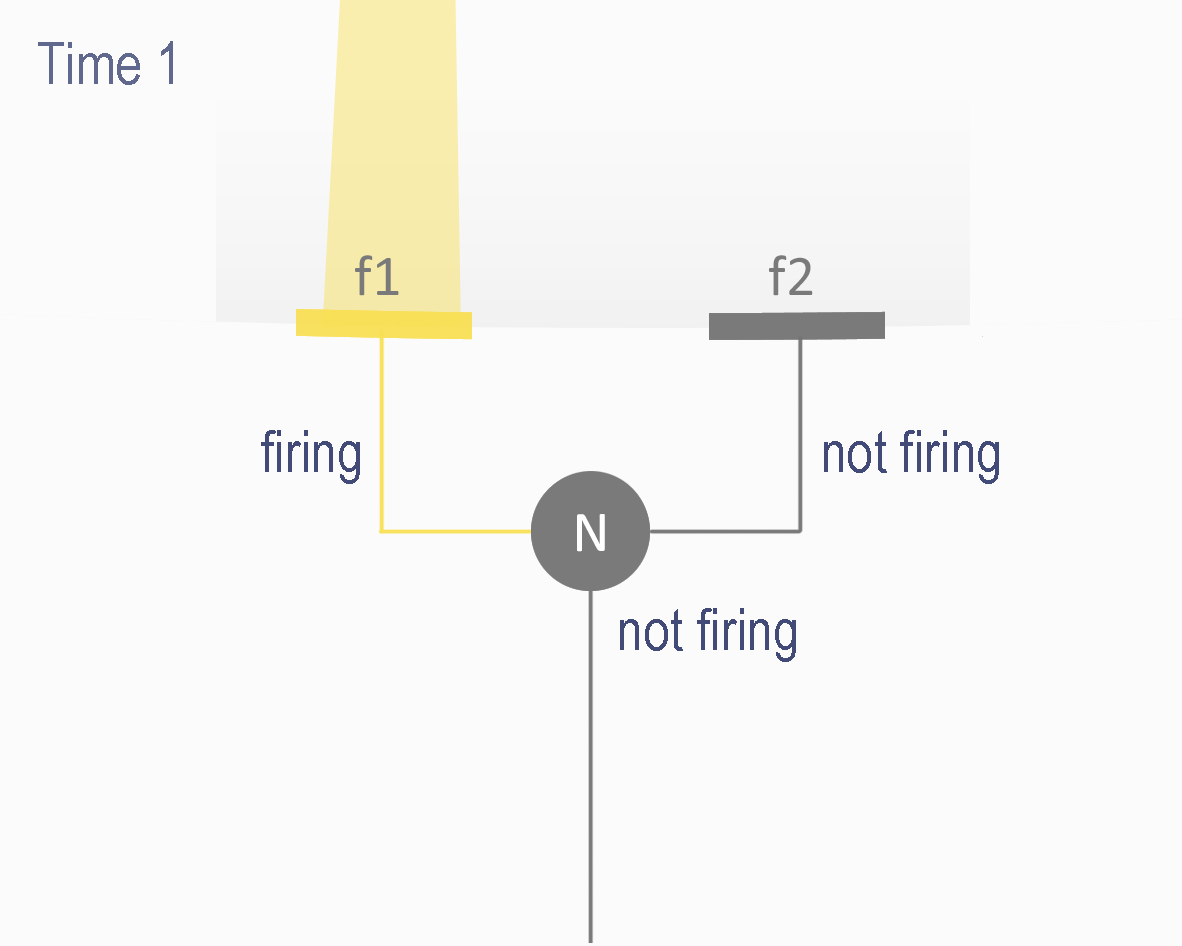
\includegraphics[width=1\linewidth]{figure/model1.png}
\columnbreak
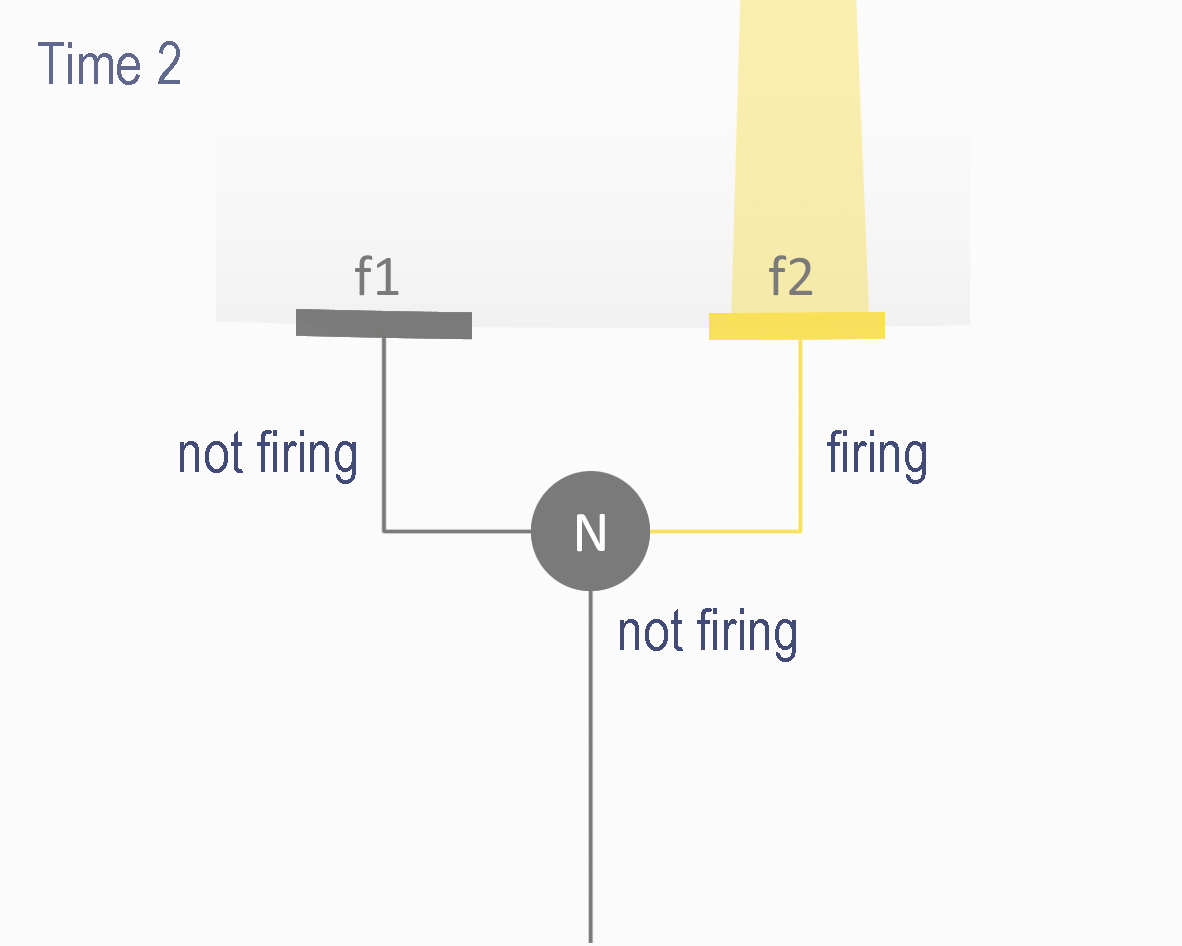
\includegraphics[width=1\linewidth]{figure/model2.png}
\end{multicols}
\caption{This circuit is unresponsive to motion between f1 and f2, as the signal need to arrive simultaneously at N for it to fire.}
\label{fig:nodelay}
\end{figure}
Werner \cite{beetle} noted that such a system would respond to motion if the signal from f1 took longer time to reach N, compared to the signal from f2. This delay could be implemented a number of ways, such as by having longer "wires", between f1 and N. Figure \ref{fig:delay}, represents the system from above but with a delay between f1 and N. As before f1 still fires first, but it does not reach N immediately. When f2 fire, f1's signal is still heading towards N, and the signals now reach N at the same time. Neuron N now fire, signaling motion. There are a few things to note. (1) the delay is static. As such, each particular circuit is attuned to a specific speed. (2) f1 and f2 do not move, as such N only detects movement in a certain direction. (3) because the responses of the fields are dependent upon the moving object's brightness, N can not distinguish between a bright object moving at an angle between the fields, and a dim object moving in the direction N is sensitive to. (4) If a large  object cover both f1, and f2, both will fire so long as the object is in front of them, meaning that N will fire event if there no motion in a large object.
\begin{figure}[H]
\begin{multicols}{2}
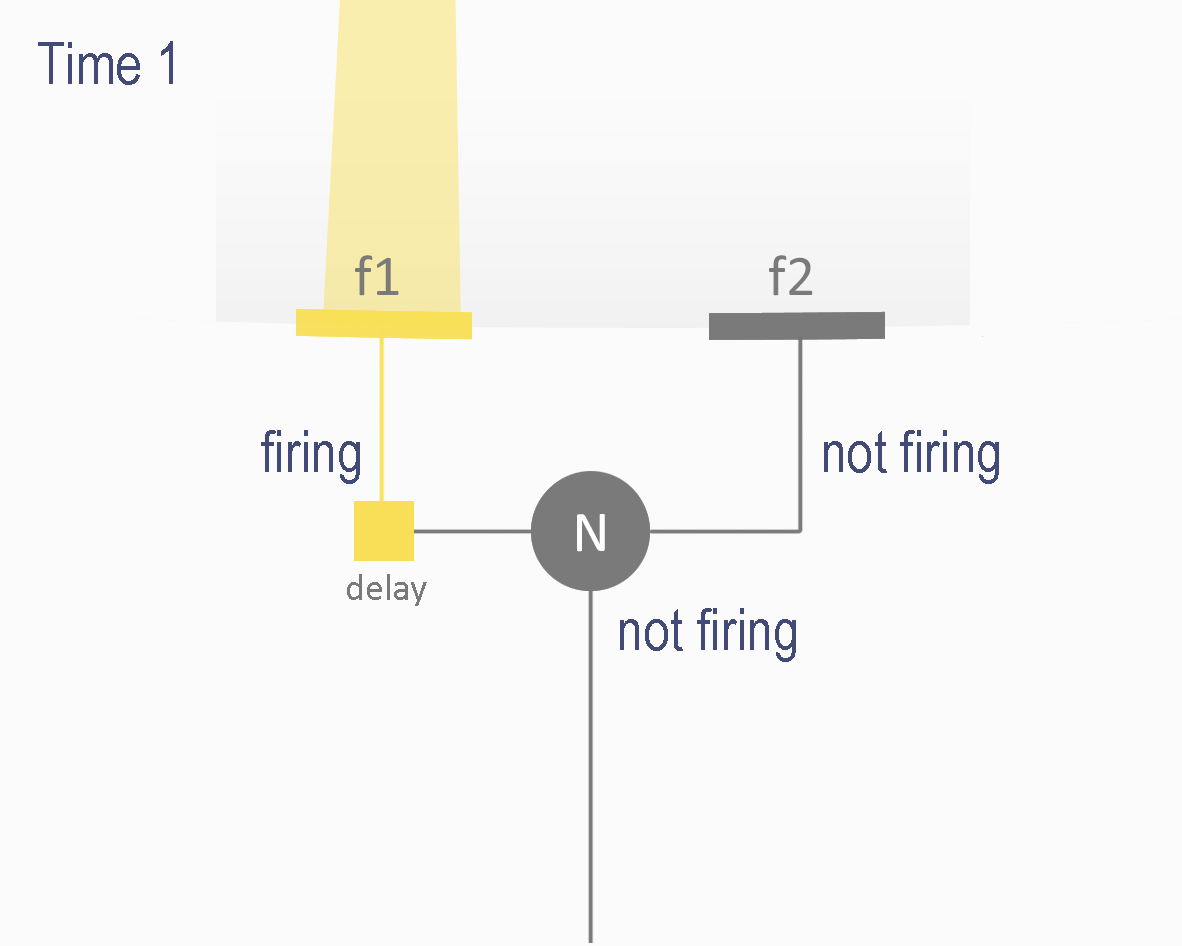
\includegraphics[width=1\linewidth]{figure/model3.png}
\columnbreak
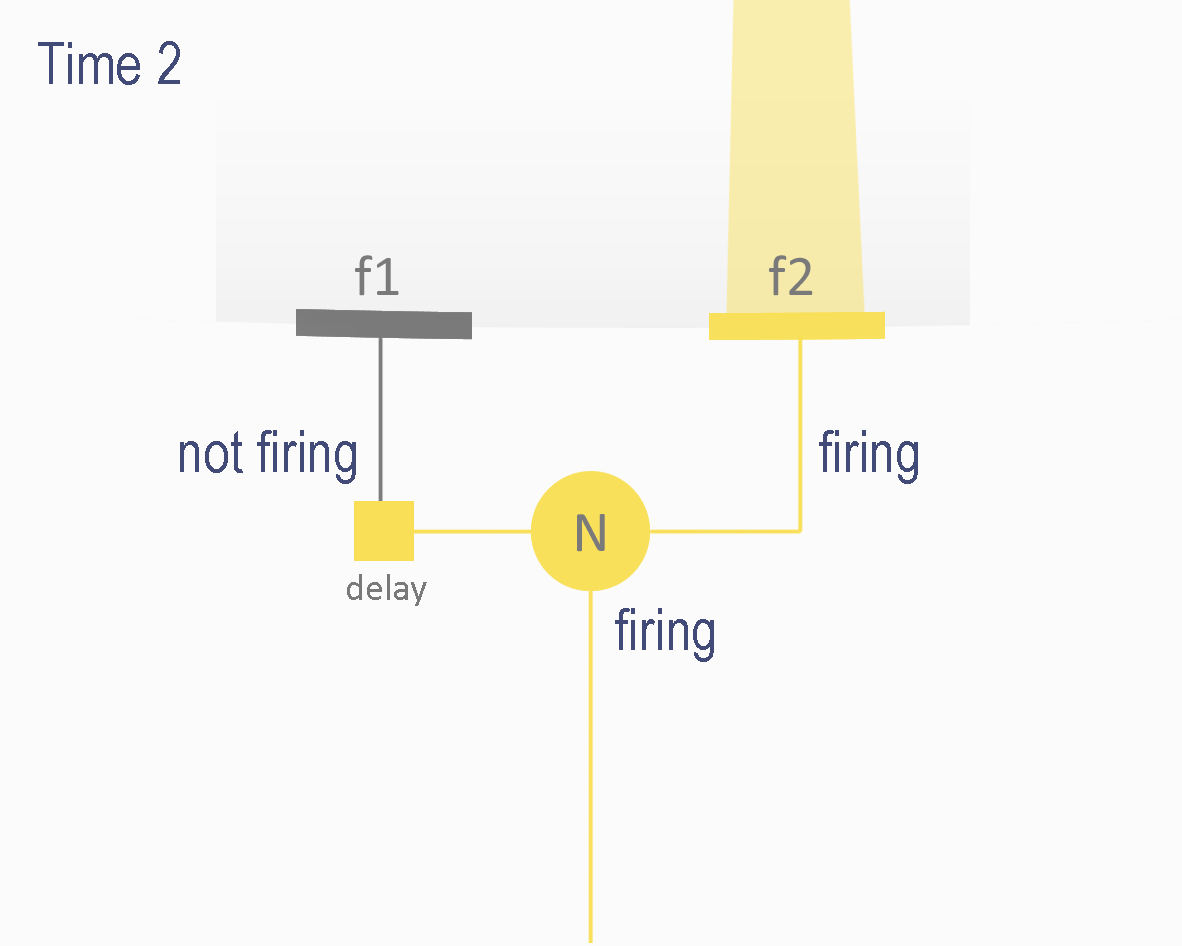
\includegraphics[width=1\linewidth]{figure/model4.png}
\end{multicols}
\caption{By introducing a delay between f1 and N, The system now responsd to motion between f1 and f2. However, this system is sensitive a particular speed. A point moves too fast, and the signal from f2 will reach N before the one from f1, and if too slow it will reach N after f1's signal.}
\label{fig:delay}
\end{figure}
These problems have led to the suggesting that these types of circuits operate in pairs of two. With two neurons (N1 and N2) sensitive to motion in opposite direction as shown in Figure \ref{fig:final}. In this circuit the final output OUT is a neuron which normally fires at a baseline rate. OUT get an excitatory signal, which causes it to fire more often, from N2, and an inhibitory which causes it to fire less often from N1. In other words, if N2 fires the output will be larger, and if N1 fires the output will be smaller, and if none or both fire the output will be the normal baseline. This change solves some of the problems with the circuit above. (3), in cases where the objects direction is neither in N1 or N2's preferred direction, both will give a weaker signal canceling each other out. (4) In case of a stationary object, both N1 and N2 will again send a similar signal, canceling each other out.
\begin{figure}[H]
\begin{multicols}{2}
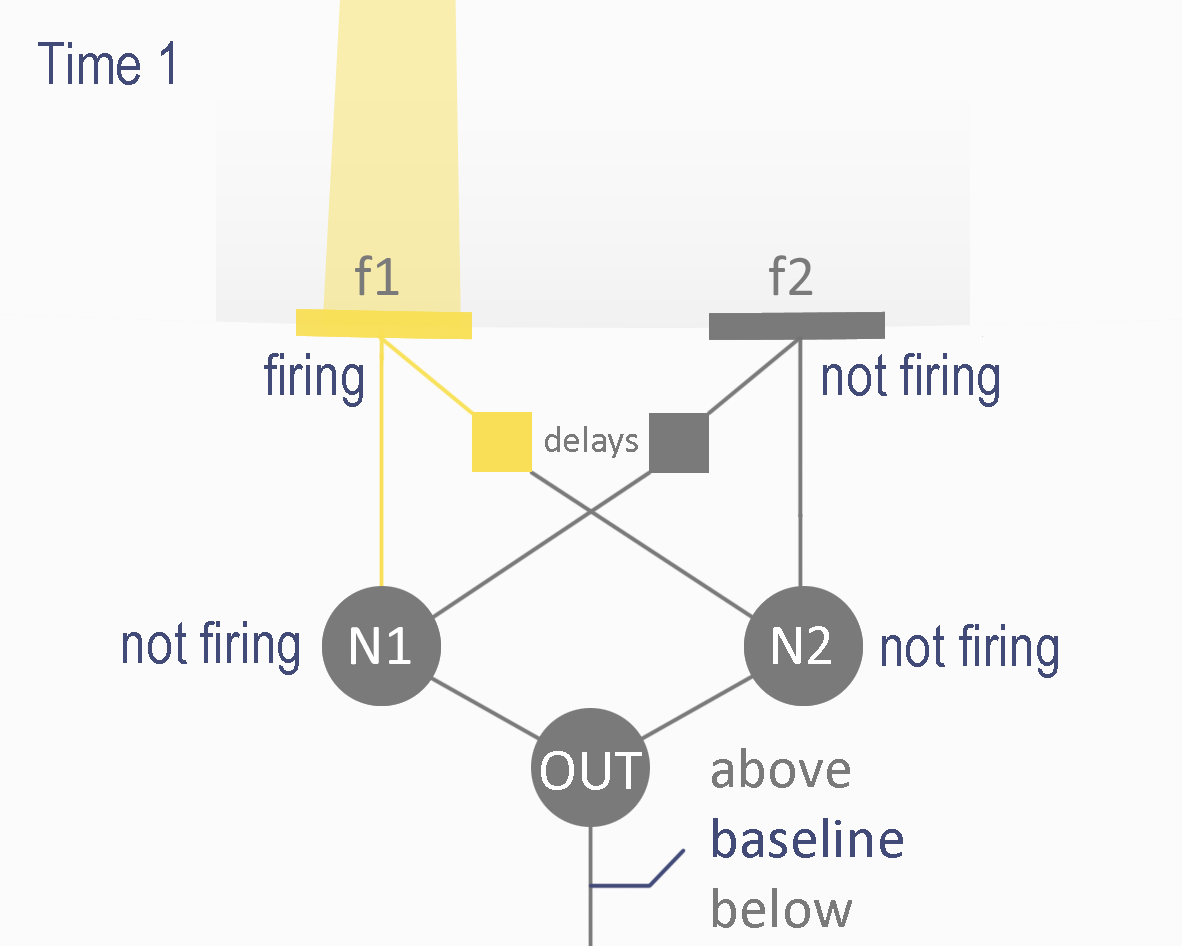
\includegraphics[width=1\linewidth]{figure/model5.png}
\columnbreak
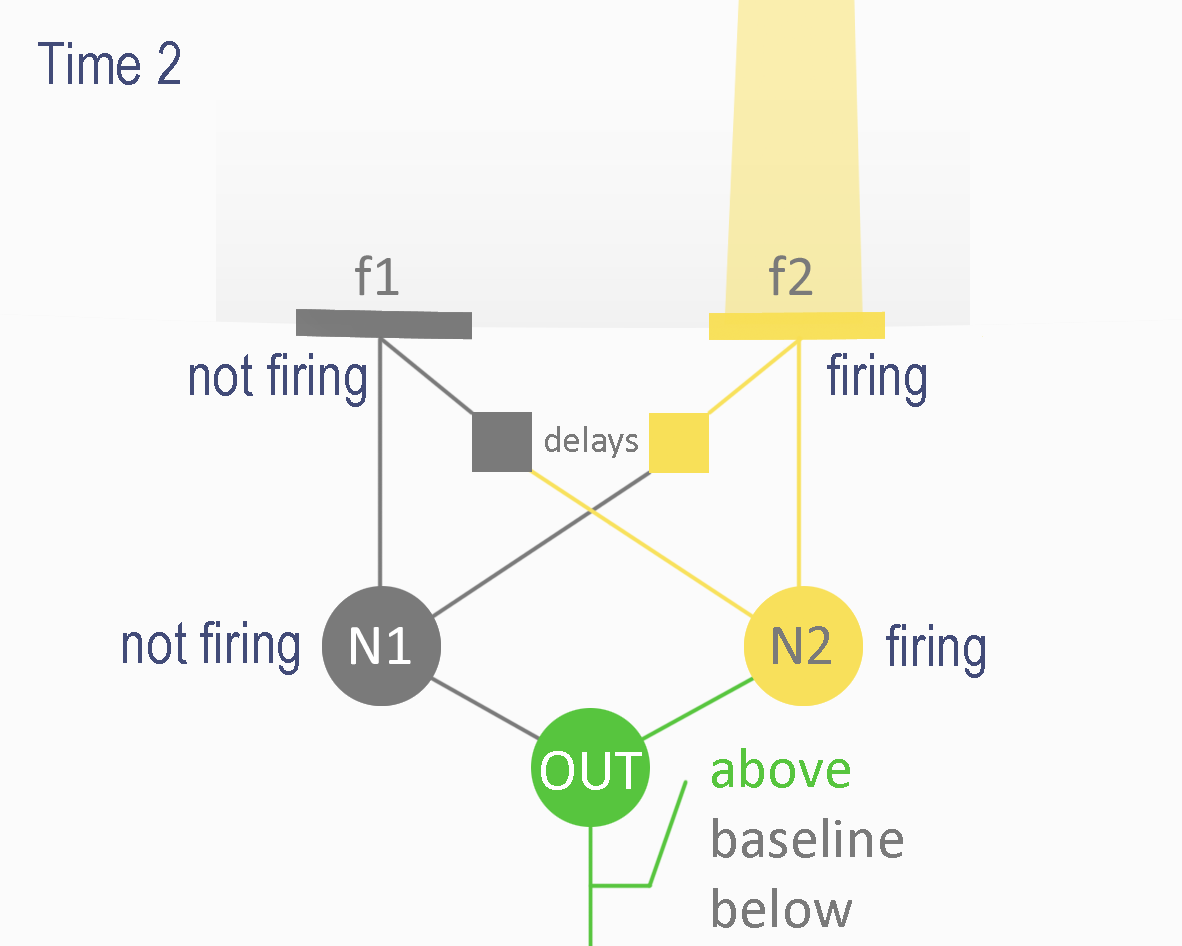
\includegraphics[width=1\linewidth]{figure/model6.png}
\end{multicols}
\caption{WIP figure text missing}
\label{fig:final}
\end{figure}
This circuit has properties similar to those of the direction sensitive cells in rabbit eyes described by \cite{Barlow1965}. If a stimulus is moved over f1 and f2 in succession. N2 will fire and N1 will not, resulting in a big output when luminance changes happens in the preferred direction. Reverse the direction, so that f2 gets hit first, and only a inhibitory signal is fired, resulting in a smaller than baseline output.
\section{Optic flow as a mechanism for illusory self motion}
Knowing that optic flow is important for movement perception, goes a long way to explaining the phenomenon of vection. Let us again consider the train scene. If one is sitting in a stationary train, and the train outside the window sets in motion, the train will be moving on the retina in a way reminiscent of optical flow. It will stimulate the eyes in ways similar to optical flow. The input to the brain is the same as if actual motion happened and the brain can not differentiate between the simulated and real optical flow. For the brain, the presence of flow indicates motion and the direction of the flow indicates movement in the opposite direction.\\\\
But the motion system is based on a large range of factors input from different modalities, such as visual, auditory, vestibular, somatosensory, and proprioceptive systems (\cite{wind}). With your eyes closed you can very easily tell weather you are moving or not. I know that this is stating the obvious but it illustrates that there are other processes that normally would prevent optic flow from tricking the brain. Therefore, one is more likely to experience vection in situations where these other stimuli are absent. Take as an example the train. Passengers are in an enclosed space, and so do not feel air resistance during motion. This would normally clue the brain into whether you or the background is moving. The movement of the train is independent from your muscles. So the signals sent to the motor neurons in the muscle so there is no help to get from the vestibular system. You are effectively stationary in a moving box, neither your balance or perception of where your limbs are(proprioception) indicates whether you are in motion. All this is to say that the range of situations in which one can experience vection is quiet limited. Most people experience vection when around or aboard vehicles large enough to alter optic flow, and shield them from the elements.\\\\
When vection causes a feeling of movement in a straight line it is called \textit{linear vection}(\cite{vectionlinear}). Other types of vection exist that can be experienced under different conditions. When placed inside a rotating drum with patterns, people experience a different type of vection called circular vection. This is used mostly in experimental studies, as these conditions rarely occur in real life.
The strength of the vection is dependant upon a number of factors such as the size of the flow, with larger motion causing a more compelling illusion. The further away the flow is perceived as being, the better it is at inducing vection. Meaning that optic flow in the peripheral vision is more likely to cause vection. This is supported by \cite{vection}, who found that when inducing vection, movement in the background was dominant over foreground movement.\\\\\todo{figure}
The duration of vection depends on the environment that caused it. In lab conditions specifically designed for it, and with continuous stimuli vection can last for ten's of seconds(\cite{vection}). But in real world scenarios vection will rarely last this long.  
\section{Vection in relation to other types of illusory self motion}
\cite{challenges}, points out that the illusion of self motion can be achieved by stimulating many different areas. for example, using auditory cues illusory movement can be induced, though they tend to be weaker than visual illusions (\cite{auditory, movement}). \cite{wind} found that wind hitting a large of the body could induce illusions of self movement. Even simple biomechanical movement can induce illusion of self motion (\cite{movement,challenges}). At the end of the day, how vection is different from the above mentioned illusion really depend on how you define it. As mentioned in section \ref{sec:def}, there are multiple definitions of vection. In many of the studies cited they use  vection to describe their respective illusion. So whether or not they are part of vection depends on who you ask. Based on the definition used in this paper, Vection differs from other type of illusory motion, in that it is caused solely through exposure to optic flow. 
\section{Discussion}
Vection is a topic of particular interest for people working with different types of virutal reality, as is appears to be linked to visually induced motion sickness(VIMS)(\cite{vims}). It is a fact that VIMS almost never occur without vection, though whether it shields against or worsen the effect of VIMS is currently unknown. It also seems that conditions that are more likely to cause VIMS also are more likely to induce vection. And further research into 
VECTION AND VR, roller coasters
Visually induced motion sickness

\bibliographystyle{apacite}
\bibliography{include/backmatter/bibliography}

\end{document}